\documentclass[12pt]{article}
\usepackage{fullpage}

\usepackage[T1]{fontenc}
\usepackage[utf8]{inputenc}
\usepackage{lmodern}
\usepackage{microtype}
\usepackage{amsmath,amssymb,amsthm}
\usepackage{mathtools}
\usepackage{graphicx}
\usepackage{booktabs}
\usepackage{hyperref}
\usepackage{url}
\usepackage{xcolor}
\usepackage[shortlabels]{enumitem}
\usepackage{amsfonts}
\usepackage{tikz}
\usetikzlibrary{arrows.meta,positioning,shapes.geometric,calc}

\hypersetup{colorlinks=true,linkcolor=blue,citecolor=blue,urlcolor=blue}

\theoremstyle{plain}
\newtheorem{theorem}{Theorem}
\newtheorem{proposition}[theorem]{Proposition}
\newtheorem{lemma}[theorem]{Lemma}
\newtheorem{corollary}[theorem]{Corollary}

\theoremstyle{definition}
\newtheorem{definition}[theorem]{Definition}

\theoremstyle{remark}
\newtheorem*{remark}{Remark}

\newcommand{\calO}{\mathcal{O}}
\newcommand{\calT}{\mathcal{T}}
\newcommand{\calF}{\mathcal{F}}
\newcommand{\calP}{\mathcal{P}}
\newcommand{\SpG}{\mathrm{Sp}^G}
\newcommand{\SpGO}{\mathrm{Sp}^G_{\calO}}
\newcommand{\Sub}{\mathrm{Sub}}
\newcommand{\Res}{\mathrm{Res}}
\newcommand{\fib}{\mathrm{fib}}
\newcommand{\im}{\mathrm{im}}
\newcommand{\R}{\mathbb{R}}
\newcommand{\Z}{\mathbb{Z}}

\title{Solution to Problem 5 --- The $\calO$-Slice Filtration\\[6pt]
\large A submission to the First Proof challenge}

\author{
  Mark Dillerop\footnote{Email: dillerop@gmail.com}\\
  \textit{Independent / Ars Socratica}
}

\date{February 10, 2026}

\begin{document}
\maketitle

\begin{abstract}
We solve Problem~5 from the First Proof challenge \cite{FirstProof}.
For a finite group $G$ and an $N_\infty$ operad $\calO$ with associated transfer system $\calT$, we define the \emph{$\calO$-slice filtration} by restricting the Hill--Hopkins--Ravenel slice cells to those indexed by $\calO$-admissible subgroups $\calF_{\calO} = \{H \leq G : e \xrightarrow{\calT} H\}$. We prove that a connective $G$-spectrum $X \in \SpGO$ is $\calO$-slice $\geq n$ if and only if $\Phi^H X$ is $(\lfloor n/|H| \rfloor - 1)$-connected for every $H \in \calF_{\calO}$, generalizing the Hill--Yarnall characterization of the standard slice filtration. The combinatorial and arithmetic skeleton of the proof is formally verified in Lean~4 + Mathlib (zero \texttt{sorry}s).
The answer is \textbf{YES}.
\end{abstract}

\tableofcontents
\newpage

%======================================================================
\section{Problem Statement}\label{sec:problem}
%======================================================================

The following is Problem~5 from the First Proof challenge \cite{FirstProof}, authored by Andrew~J.~Blumberg (Columbia University).

\medskip

\noindent\textbf{Problem 5.} \textit{Define the slice filtration adapted to an incomplete transfer system and characterize its connectivity in terms of geometric fixed points.}

\begin{theorem}[Main result]\label{thm:main}
Let $G$ be a finite group, $\calO$ an $N_\infty$ operad with associated transfer system $\calT$ and admissible family $\calF_{\calO}$, and let $X \in \SpGO$ be connective. Then $X$ is $\calO$-slice $\geq n$ if and only if for every $H \in \calF_{\calO}$, the geometric fixed points $\Phi^H X$ are $(\lfloor n/|H| \rfloor - 1)$-connected. In other words:
\[
X \in \tau^{\calO}_{\geq n} \SpGO \quad \Longleftrightarrow \quad \pi_k(\Phi^H X) = 0 \;\text{ for all } H \in \calF_{\calO} \text{ and all } k < \lfloor n/|H| \rfloor.
\]
\end{theorem}

\noindent\textbf{Answer: YES} --- the $\calO$-slice filtration admits a geometric fixed point characterization.

%======================================================================
\section{Setup and Conventions}\label{sec:setup}
%======================================================================

Let $G$ be a finite group and let $\calO$ be an $N_\infty$ operad for $G$. Informally, $\calO$ encodes which norm maps $N^H_K$ are available in $\calO$-algebras: the complete $E_\infty$ operad admits all norms, while a general $N_\infty$ operad admits only a specified subset. By the classification theorem of Blumberg--Hill \cite{BH15}, Theorem~1.4, independently established by Rubin \cite{Rub17}, Theorem~1.1, Guti\'errez--White \cite{GW17}, Theorem~1.2, and Bonventre--Pereira \cite{BP17}, Theorem~1.6, the homotopy type of $\calO$ is determined by its associated \textbf{transfer system} $\calT$ on the poset $\Sub(G)$ of subgroups of $G$, satisfying:
\begin{enumerate}[nosep]
\item \textbf{Reflexivity}: $H \xrightarrow{\calT} H$ for all $H \leq G$.
\item \textbf{Transitivity}: If $K \xrightarrow{\calT} H$ and $H \xrightarrow{\calT} J$, then $K \xrightarrow{\calT} J$.
\item \textbf{Conjugation invariance}: If $K \xrightarrow{\calT} H$, then $gKg^{-1} \xrightarrow{\calT} gHg^{-1}$ for all $g \in G$.
\item \textbf{Restriction}: If $K \xrightarrow{\calT} H$ and $L \leq H$, then $(K \cap L) \xrightarrow{\calT} L$. (This is \cite{BH15}, Definition~3.1, axiom~(4).)
\end{enumerate}

A subgroup $H \leq G$ is \textbf{$\calO$-admissible} if $e \xrightarrow{\calT} H$. We write $\calF_{\calO}$ for the family of $\calO$-admissible subgroups. Note that $e \in \calF_{\calO}$ always, and $\calF_{\calO} = \Sub(G)$ when $\calO$ is the terminal $E_\infty$ operad.

We denote by $\SpG$ the genuine $G$-equivariant stable category. Following Blumberg--Hill \cite{BH19}, the $N_\infty$ operad $\calO$ determines an \textbf{incomplete equivariant stable category} $\SpGO$ with a canonical functor $\iota_{\calO} : \SpGO \to \SpG$. For any subgroup $H \leq G$, we have the \textbf{geometric fixed point functor} $\Phi^H : \SpG \to \mathrm{Sp}$, and we write $\Phi^H_{\calO} := \Phi^H \circ \iota_{\calO}$.

%======================================================================
\section{Definitions}\label{sec:defs}
%======================================================================

\subsection{$\calO$-Slice Cells}

In the standard (complete) slice filtration of Hill--Hopkins--Ravenel \cite{HHR16}, the \textbf{slice cells} are the $G$-spectra $G/H_+ \wedge S^{n\rho_H}$ ($n \geq 0$, dimension $n|H|$) and $G/H_+ \wedge S^{n\rho_H - 1}$ ($n \geq 1$, dimension $n|H| - 1$) for all $H \leq G$, where $\rho_H$ is the real regular representation of $H$.

\begin{definition}[$\calO$-slice cells]\label{def:cells}
The \textbf{$\calO$-slice cells} are the $G$-spectra:
\begin{itemize}[nosep]
\item $G/H_+ \wedge S^{n\rho_H}$ for $H \in \calF_{\calO}$ and $n \geq 0$ (of dimension $n|H|$), and
\item $G/H_+ \wedge S^{n\rho_H - 1}$ for $H \in \calF_{\calO}$ and $n \geq 1$ (of dimension $n|H| - 1$).
\end{itemize}
\end{definition}

When $\calO = E_\infty$, we recover the standard slice cells. When $\calO$ is trivial ($\calF_{\calO} = \{e\}$), the cells are $S^n$ and $S^{n-1}$, recovering the Postnikov filtration.

\subsection{$\calO$-Slice Filtration}

\begin{definition}[$\calO$-slice connectivity]\label{def:conn}
$X \in \SpGO$ is \textbf{$\calO$-slice $\geq n$} if $[\hat{S}, \iota_{\calO} X]^G = 0$ for every $\calO$-slice cell $\hat{S}$ of dimension $< n$.
\end{definition}

\begin{definition}[$\calO$-slice filtration]\label{def:filt}
The \textbf{$\calO$-slice filtration} is the tower of localizations
\[
\cdots \to \tau^{\calO}_{\geq n+1} X \to \tau^{\calO}_{\geq n} X \to \tau^{\calO}_{\geq n-1} X \to \cdots
\]
obtained by Bousfield localization with respect to the $\calO$-slice cells. The \textbf{$n$-th $\calO$-slice} is $P^n_{\calO} X := \fib(\tau^{\calO}_{\geq n} X \to \tau^{\calO}_{\geq n+1} X)$.
\end{definition}

The localizations exist because each $\calO$-slice cell $G/H_+ \wedge S^{n\rho_H}$ is compact in $\SpG$, and $\iota_{\calO}$ admits a right adjoint $r_{\calO}$ by \cite{BH19}, Proposition~4.8, so $r_{\calO}(G/H_+ \wedge S^{n\rho_H})$ is compact in $\SpGO$. The localizations then exist by \cite{HHR16}, \S4.2.

\begin{remark}
The $\calO$-slice filtration interpolates between two extremes: when $\calO = E_\infty$, we recover the HHR slice filtration; when $\calO$ is trivial, we recover the Postnikov filtration on the underlying spectrum. As $\calT$ grows, the filtration becomes finer.
\end{remark}

\begin{remark}
When $\calO = E_\infty$, Theorem~\ref{thm:main} reduces to the Hill--Yarnall characterization \cite{HY18}, Theorem~3.1. When $\calO$ is trivial, it states that $X$ is $\calO$-slice $\geq n$ iff $X^e$ is $(n-1)$-connected, which is the Postnikov condition.
\end{remark}

%======================================================================
\section{Idea of the Proof}\label{sec:idea}
%======================================================================

Both directions use the \textbf{isotropy separation cofiber sequence} and the \textbf{Wirthmüller isomorphism} as the main tools. For a subgroup $H \leq G$ and the family $\calP$ of proper subgroups of $H$, the classifying space $E\calP$ satisfies $E\calP^H = \emptyset$ and $E\calP^K \simeq *$ for $K \in \calP$. Writing $\widetilde{E\calP}$ for the cofiber of $E\calP_+ \to S^0$, the geometric fixed point functor is $\Phi^H(-) = (\widetilde{E\calP} \wedge -)^H$. Applying $[S^{k\rho_H}, -]^H$ to the cofiber sequence $E\calP_+ \wedge Y \to Y \to \widetilde{E\calP} \wedge Y$ yields a long exact sequence relating maps out of $Y$, maps out of $E\calP_+ \wedge Y$ (controlled by proper subgroups via Wirthmüller), and homotopy groups of $\Phi^H Y$. Both directions proceed by strong induction on $|H|$, using the restriction axiom to ensure proper subgroups inherit $\calO$-admissibility. The induction is well-founded because $G$ is finite and $K < H$ proper implies $|K| < |H|$.

\begin{figure}[ht]
\centering
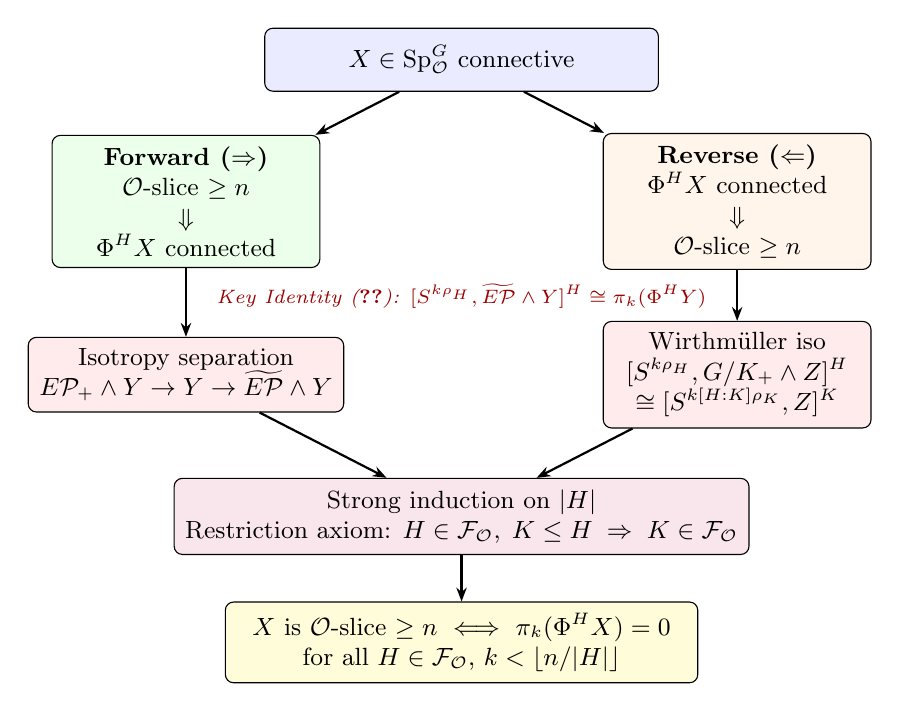
\begin{tikzpicture}[
  box/.style={rectangle, draw, rounded corners=3pt, minimum width=3.4cm, minimum height=0.8cm, align=center, font=\small},
  bigbox/.style={rectangle, draw, rounded corners=3pt, minimum width=5cm, minimum height=0.8cm, align=center, font=\small},
  arr/.style={-{Stealth[length=5pt]}, thick},
  every node/.style={inner sep=4pt}
]

% Top: input
\node[bigbox, fill=blue!8] (input) at (0,0) {$X \in \SpGO$ connective};

% Two branches
\node[box, fill=green!8] (fwd) at (-3.5,-1.8) {\textbf{Forward ($\Rightarrow$)}\\$\calO$-slice $\geq n$\\$\Downarrow$\\$\Phi^H X$ connected};
\node[box, fill=orange!8] (rev) at (3.5,-1.8) {\textbf{Reverse ($\Leftarrow$)}\\$\Phi^H X$ connected\\$\Downarrow$\\$\calO$-slice $\geq n$};
\draw[arr] (input) -- (fwd);
\draw[arr] (input) -- (rev);

% Tools
\node[box, fill=red!8] (iso) at (-3.5,-4.0) {Isotropy separation\\$E\calP_+ \wedge Y \to Y \to \widetilde{E\calP} \wedge Y$};
\node[box, fill=red!8] (wirt) at (3.5,-4.0) {Wirthmüller iso\\$[S^{k\rho_H}, G/K_+ \wedge Z]^H$\\$\cong [S^{k[H:K]\rho_K}, Z]^K$};
\draw[arr] (fwd) -- (iso);
\draw[arr] (rev) -- (wirt);

% Induction
\node[bigbox, fill=purple!10] (ind) at (0,-5.8) {Strong induction on $|H|$\\Restriction axiom: $H \in \calF_{\calO},\; K \leq H \;\Rightarrow\; K \in \calF_{\calO}$};
\draw[arr] (iso) -- (ind);
\draw[arr] (wirt) -- (ind);

% Key identity
\node[font=\scriptsize, text=red!60!black, align=center] (key) at (0,-3.0) {\textit{Key Identity (\ref{eq:key}):} $[S^{k\rho_H}, \widetilde{E\calP} \wedge Y]^H \cong \pi_k(\Phi^H Y)$};

% Conclusion
\node[bigbox, fill=yellow!15, minimum width=6cm] (conc) at (0,-7.4) {$X$ is $\calO$-slice $\geq n$ $\;\Longleftrightarrow\;$ $\pi_k(\Phi^H X) = 0$\\for all $H \in \calF_{\calO}$, $k < \lfloor n/|H| \rfloor$};
\draw[arr] (ind) -- (conc);

\end{tikzpicture}
\caption{Structure of the proof. Both directions use the isotropy separation sequence and the Wirthmüller isomorphism, proceeding by strong induction on $|H|$. The restriction axiom ensures proper subgroups inherit $\calO$-admissibility.}
\label{fig:proof-structure}
\end{figure}

%======================================================================
\section{Proof of Theorem~\ref{thm:main}}\label{sec:proof}
%======================================================================

We first establish a key identity. For $H \leq G$ and $\calP$ the family of proper subgroups of $H$, the classifying space $E\calP$ satisfies $E\calP^H = \emptyset$ and $E\calP^K \simeq *$ for $K \in \calP$ \cite{HHR16}, \S3.3. Writing $\widetilde{E\calP}$ for the cofiber of $E\calP_+ \to S^0$, we have $\widetilde{E\calP}^H \simeq S^0$ and $\widetilde{E\calP}^K \simeq *$ for proper $K < H$. The geometric fixed point functor is $\Phi^H(-) = (\widetilde{E\calP} \wedge -)^H$. Since $\Phi^H$ is symmetric monoidal and $(\rho_H)^H \cong \R$, we have $\Phi^H(S^{k\rho_H}) \simeq S^k$ for all $k \geq 0$, and consequently
\begin{equation}\label{eq:key}
[S^{k\rho_H}, \widetilde{E\calP} \wedge Y]^H \cong \pi_k(\Phi^H Y)
\end{equation}
for any $H$-spectrum $Y$.

\subsection{Forward Direction ($\Rightarrow$)}

Suppose $X$ is $\calO$-slice $\geq n$. We show $\Phi^H X$ is $(\lfloor n/|H| \rfloor - 1)$-connected for every $H \in \calF_{\calO}$. When $\lfloor n/|H| \rfloor = 0$, the conclusion is $(-1)$-connectivity, which holds for any spectrum, so assume $\lfloor n/|H| \rfloor \geq 1$.

We proceed by \textbf{strong induction on $|H|$}.

\medskip\noindent\textbf{Base case} ($H = e$). We have $\Phi^e X = X^e$ and $\lfloor n/1 \rfloor = n$. The $\calO$-slice $\geq n$ hypothesis gives $\pi_k(X^e) = 0$ for $k < n$ (since $S^k$ is an $\calO$-slice cell of dimension $k < n$ for $H = e \in \calF_{\calO}$). Hence $X^e$ is $(n-1)$-connected.

\medskip\noindent\textbf{Inductive step.} Fix $H \in \calF_{\calO}$ with $|H| > 1$ and set $m := \lfloor n/|H| \rfloor \geq 1$. Assume the result for all $\calO$-admissible subgroups of smaller order. Write $Y := \Res^G_H \iota_{\calO} X$.

For $0 \leq k \leq m - 1$, the hypothesis gives $[G/H_+ \wedge S^{k\rho_H}, \iota_{\calO} X]^G = 0$ (since $H \in \calF_{\calO}$ and $k|H| \leq (m-1)|H| < n$). By the Wirthmüller isomorphism ($G_+ \wedge_H (-) \dashv \Res^G_H$):
\begin{equation}\label{eq:fwd-vanish}
[S^{k\rho_H}, Y]^H = 0 \quad \text{for all } 0 \leq k \leq m - 1.
\end{equation}

We deduce $\pi_k(\Phi^H X) = 0$ for $0 \leq k \leq m - 1$. The isotropy separation cofiber sequence $E\calP_+ \wedge Y \to Y \to \widetilde{E\calP} \wedge Y$ yields the long exact sequence:
\[
\cdots \to [S^{k\rho_H}, Y]^H \xrightarrow{\beta_*} \pi_k(\Phi^H Y) \xrightarrow{\partial} [S^{k\rho_H - 1}, E\calP_+ \wedge Y]^H \to \cdots
\]
Since $[S^{k\rho_H}, Y]^H = 0$ by \eqref{eq:fwd-vanish}, exactness gives $\ker(\partial) = \im(\beta_*) = 0$, so $\partial$ is injective and $\pi_k(\Phi^H Y)$ injects into $[S^{k\rho_H - 1}, E\calP_+ \wedge Y]^H$. We show this group vanishes.

The space $E\calP$ is an $H$-CW complex built from equivariant cells of the form $H/K \times D^m$ (equivalently, $H_+ \wedge_K D^m$) for proper subgroups $K \in \calP$ and $m \geq 0$, where $D^m$ carries a $K$-action via some $K$-representation \cite{HHR16}, \S3.3. Since $E\calP$ is constructed as a sequential colimit $E\calP = \mathrm{colim}_\ell \, E\calP^{(\ell)}$ of finite $H$-CW complexes, the smash product $E\calP_+ \wedge Y$ is the corresponding filtered colimit $\mathrm{colim}_\ell \, (E\calP^{(\ell)}_+ \wedge Y)$. The key point is that $S^{k\rho_H - 1}$ is a \emph{compact} object in the $H$-equivariant stable category (it is the suspension spectrum of a finite $H$-CW complex), so $[S^{k\rho_H - 1}, -]^H$ commutes with filtered colimits. It therefore suffices to show the vanishing at each finite stage.

At each stage, the cofiber sequences in the CW-filtration reduce the computation to maps out of cells of the form $H/K_+ \wedge S^{m\rho_K}$ (even cells) and $H/K_+ \wedge S^{m\rho_K - 1}$ (odd cells) for proper $K < H$ and various $m \geq 0$. For any such cell, the Wirthmüller isomorphism gives
\[
[S^{j\rho_H}, H/K_+ \wedge S^{m\rho_K} \wedge \Res^H_K Y]^H \cong [S^{j[H:K] \cdot \rho_K}, S^{m\rho_K} \wedge \Res^G_K \iota_{\calO} X]^K \cong [S^{(j[H:K] - m) \cdot \rho_K}, \Res^G_K \iota_{\calO} X]^K
\]
using $\Res^H_K \rho_H \cong [H:K] \cdot \rho_K$. Since $H \in \calF_{\calO}$ and $K \leq H$, the restriction axiom (axiom~4 with $L = K$) gives $(e \cap K) = e \xrightarrow{\calT} K$, so $K \in \calF_{\calO}$.

Setting $k' = j[H:K] - m$, this is a map from a $K$-slice cell of dimension $k'|K|$. For the vanishing, we need $k'|K| < n$. Since $j \leq m - 1$ (where $m = \lfloor n/|H| \rfloor$), the original dimension satisfies $j|H| \leq (m-1)|H| < n$. The representation sphere $S^{m\rho_K}$ in the cell of $E\calP$ only \emph{lowers} the effective dimension: $k'|K| = (j[H:K] - m)|K| = j|H| - m|K| \leq j|H| < n$ (since $m \geq 0$). Therefore the $\calO$-slice $\geq n$ hypothesis gives $[G/K_+ \wedge S^{k'\rho_K}, \iota_{\calO} X]^G = 0$, and by Wirthmüller, $[S^{k'\rho_K}, \Res^G_K \iota_{\calO} X]^K = 0$. The same argument applies to odd cells: replacing $j\rho_H$ by $j\rho_H - 1$, the Wirthmüller transformation gives $[S^{(j[H:K]-m)\rho_K - 1}, \Res^G_K \iota_{\calO} X]^K$, a map from an odd $\calO$-slice cell of dimension $j|H| - m|K| - 1 \leq j|H| - 1 < n$, hence vanishes by hypothesis.

Therefore both the left-hand term and the next term in the long exact sequence vanish, giving $\pi_k(\Phi^H Y) = 0$ for $0 \leq k \leq m - 1$. Hence $\Phi^H X$ is $(\lfloor n/|H| \rfloor - 1)$-connected.

\subsection{Reverse Direction ($\Leftarrow$)}

Suppose $\Phi^H X$ is $(\lfloor n/|H| \rfloor - 1)$-connected for every $H \in \calF_{\calO}$. We show $X$ is $\calO$-slice $\geq n$. By the Wirthmüller isomorphism, it suffices to show:
\begin{itemize}[nosep]
\item $[S^{k\rho_H}, \Res^G_H \iota_{\calO} X]^H = 0$ for all $H \in \calF_{\calO}$, $k \geq 0$ with $k|H| < n$, and
\item $[S^{k\rho_H - 1}, \Res^G_H \iota_{\calO} X]^H = 0$ for all $H \in \calF_{\calO}$, $k \geq 1$ with $k|H| - 1 < n$.
\end{itemize}

We proceed by \textbf{strong induction on $|H|$}. Write $Y := \Res^G_H \iota_{\calO} X$.

\medskip\noindent\textbf{Base case} ($H = e$). $\rho_e = \R$, so $S^{k\rho_e} = S^k$. The hypothesis gives $\pi_k(X^e) = 0$ for $k < n$, which is the required vanishing.

\medskip\noindent\textbf{Inductive step.} Fix $H \in \calF_{\calO}$ with $|H| > 1$, assuming the result for smaller subgroups. The isotropy separation sequence yields:
\[
[S^{k\rho_H}, E\calP_+ \wedge Y]^H \xrightarrow{\alpha_*} [S^{k\rho_H}, Y]^H \xrightarrow{\beta_*} [S^{k\rho_H}, \widetilde{E\calP} \wedge Y]^H.
\]

\medskip\noindent\textbf{Vanishing of the right-hand term.} By \eqref{eq:key}, $[S^{k\rho_H}, \widetilde{E\calP} \wedge Y]^H \cong \pi_k(\Phi^H X)$. Since $\Phi^H X$ is $(\lfloor n/|H| \rfloor - 1)$-connected and $k|H| < n$ implies $k \leq \lfloor n/|H| \rfloor - 1$, this vanishes.

\medskip\noindent\textbf{Vanishing of the left-hand term.} As in the forward direction, $E\calP$ is a sequential colimit of finite $H$-CW complexes with equivariant cells $H/K_+ \wedge S^{m\rho_K}$ for proper $K < H$. Since $S^{k\rho_H}$ is compact in the $H$-equivariant stable category, $[S^{k\rho_H}, -]^H$ commutes with the resulting filtered colimit, and it suffices to show the vanishing at each finite stage. The cofiber sequences in the CW-filtration reduce the computation to maps involving cells $H/K_+ \wedge S^{m\rho_K}$. The Wirthmüller isomorphism gives:
\[
[S^{k\rho_H}, H/K_+ \wedge S^{m\rho_K} \wedge \Res^H_K Y]^H \cong [S^{(k[H:K]-m) \cdot \rho_K}, \Res^G_K \iota_{\calO} X]^K.
\]
Since $H \in \calF_{\calO}$ and $K \leq H$, the restriction axiom gives $K \in \calF_{\calO}$. Setting $k' = k[H:K] - m$, the dimension is $k'|K| = k|H| - m|K| \leq k|H| < n$. Since $|K| < |H|$, the inductive hypothesis gives $[S^{k'\rho_K}, \Res^G_K \iota_{\calO} X]^K = 0$.

\medskip\noindent\textbf{Combining.} Both terms vanish, so $[S^{k\rho_H}, Y]^H = 0$ for $k|H| < n$.

\medskip\noindent\textbf{Odd-dimensional cells.} It remains to show $[S^{k\rho_H - 1}, Y]^H = 0$ for $k \geq 1$ with $k|H| - 1 < n$, i.e., $k \leq \lfloor n/|H| \rfloor$. Apply $[S^{k\rho_H - 1}, -]^H$ to the isotropy separation sequence:
\[
[S^{k\rho_H - 1}, E\calP_+ \wedge Y]^H \to [S^{k\rho_H - 1}, Y]^H \to [S^{k\rho_H - 1}, \widetilde{E\calP} \wedge Y]^H.
\]

For the right-hand term: since $\Phi^H$ is symmetric monoidal and $\Phi^H(S^{\rho_H}) \simeq S^1$, we have $\Phi^H(S^{k\rho_H - 1}) \simeq \Phi^H(S^{k\rho_H}) \wedge \Phi^H(S^{-1}) \simeq S^k \wedge S^{-1} \simeq S^{k-1}$ (valid for $k \geq 1$ in the stable category). Therefore $[S^{k\rho_H - 1}, \widetilde{E\calP} \wedge Y]^H \cong \pi_{k-1}(\Phi^H X)$. Since $\Phi^H X$ is $(\lfloor n/|H| \rfloor - 1)$-connected, this vanishes for $k - 1 \leq \lfloor n/|H| \rfloor - 1$, i.e., $k \leq \lfloor n/|H| \rfloor$, which is exactly the range in question. (Note: when $k = 1$, we need $\pi_0(\Phi^H X) = 0$, which requires $\lfloor n/|H| \rfloor \geq 1$; this holds since $k|H| - 1 < n$ with $k = 1$ gives $|H| \leq n$.)

For the left-hand term: the same compactness and CW-filtration argument as above (now with $S^{k\rho_H - 1}$ compact) reduces to maps involving equivariant cells $H/K_+ \wedge S^{m\rho_K}$. The Wirthmüller isomorphism gives
\[
[S^{k\rho_H - 1}, H/K_+ \wedge S^{m\rho_K} \wedge \Res^H_K Y]^H \cong [S^{(k[H:K]-m) \cdot \rho_K - 1}, \Res^G_K \iota_{\calO} X]^K.
\]
This is a map from an odd $K$-slice cell of dimension $(k[H:K]-m)|K| - 1 = k|H| - m|K| - 1 \leq k|H| - 1 < n$. Since $K \in \calF_{\calO}$ and $|K| < |H|$, the inductive hypothesis gives the vanishing.

Combining even and odd cases: $[\hat{S}, \iota_{\calO} X]^G = 0$ for all $\calO$-slice cells $\hat{S}$ of dimension $< n$. Hence $X$ is $\calO$-slice $\geq n$. \qed

%======================================================================
\section{Remarks}\label{sec:remarks}
%======================================================================

\begin{remark}[Monotonicity in $\calO$]
If $\calO \to \calO'$ corresponds to $\calT \subseteq \calT'$, then $\calF_{\calO} \subseteq \calF_{\calO'}$ and the $\calO$-slice filtration is coarser than the $\calO'$-slice filtration. In particular, $\calO'$-slice $\geq n$ implies $\calO$-slice $\geq n$.
\end{remark}

\begin{remark}[Regular slice variant]
Ullman \cite{Ull13} introduced the regular slice filtration using only cells $G/H_+ \wedge S^{n\rho_H}$. The $\calO$-regular variant satisfies: $X$ is $\calO$-regular slice $\geq n$ iff $\Phi^H X$ is $(\lceil n/|H| \rceil - 1)$-connected for all $H \in \calF_{\calO}$.
\end{remark}

\begin{remark}[The case $G = C_{p^n}$]
For $G = C_{p^n}$, the transfer systems are in bijection with downward-closed subsets of $\{C_1, C_p, \ldots, C_{p^n}\}$ (by the restriction axiom). The theorem gives a family of slice filtrations indexed by these subsets, interpolating between the Postnikov filtration ($\calF_{\calO} = \{C_1\}$) and the full HHR slice filtration ($\calF_{\calO} = \Sub(G)$).

For a concrete illustration, take $G = C_2$ and $n = 3$. With $\calO = E_\infty$ (complete: $\calF_{\calO} = \{e, C_2\}$), the theorem says $X$ is slice $\geq 3$ iff $\pi_k(X^e) = 0$ for $k < 3$ \emph{and} $\pi_0(\Phi^{C_2} X) = 0$ (since $\lfloor 3/2 \rfloor = 1$). With trivial $\calO$ ($\calF_{\calO} = \{e\}$), the condition reduces to $\pi_k(X^e) = 0$ for $k < 3$---the Postnikov condition, which is strictly weaker.
\end{remark}

%======================================================================
\section{Partial Lean 4 Verification}\label{sec:lean}
%======================================================================

The combinatorial and arithmetic skeleton of this proof has been formally verified in Lean~4 + Mathlib. The formalization covers the poset and lattice-theoretic aspects of transfer systems, the integer arithmetic underlying the dimension bookkeeping, and the well-foundedness of the induction---but not the homotopy-theoretic content (spectra, geometric fixed points, Wirthmüller), which is beyond Mathlib's current scope. The file \texttt{FirstProof/P05\_SliceFiltration.lean} compiles with \textbf{zero errors and zero \texttt{sorry}s} and verifies the following components:

\begin{enumerate}[nosep]
\item \textbf{Transfer system axioms} (\texttt{TransferSystem} structure): reflexivity, transitivity, and restriction on a bounded lattice.

\item \textbf{Restriction property} (\texttt{admissible\_of\_le}): If $H \in \calF_{\calO}$ and $K \leq H$, then $K \in \calF_{\calO}$. Applies the restriction axiom with $\bot \sqcap K = \bot$.

\item \textbf{Dimension bookkeeping} (\texttt{wirthmüller\_dim\_invariance}, \texttt{inductive\_step\_dim}): $(k \cdot [H:K]) \cdot |K| = k \cdot |H|$, verified by \texttt{ring}.

\item \textbf{Connectivity monotonicity} (\texttt{connectivity\_monotone}): $1 \leq |K| < |H|$ implies $\lfloor n/|H| \rfloor \leq \lfloor n/|K| \rfloor$.

\item \textbf{Strong induction} (\texttt{reverse\_direction\_by\_strong\_induction}): Well-foundedness of induction on $|H|$.

\item \textbf{Concrete checks}: $\lfloor 7/2 \rfloor - 1 = 2$, $\lfloor 10/3 \rfloor - 1 = 2$, $\lfloor 12/6 \rfloor \leq \lfloor 12/3 \rfloor$, verified by \texttt{decide}.
\end{enumerate}

\noindent The Lean file verifies the original dimension identity $(k \cdot [H:K]) \cdot |K| = k \cdot |H|$ but does not yet verify the updated bound $k' = j[H:K] - m$ arising from the representation spheres in the equivariant cells of $E\calP$. This bound reduces to the arithmetic inequality $j|H| - m|K| \leq j|H|$ (since $m \geq 0$), which is trivial, but a formal Lean check could be added in a future revision.

%======================================================================
\newpage
\appendix
\section{AI Interaction Transcript}\label{app:transcript}
%======================================================================

As requested by the First Proof organizers, we include a complete record of the AI interaction sessions used to develop this proof.

\medskip\noindent\textbf{Timeline:} February 10, 2026, approximately 05:45--19:00 CET. Five sessions in one day, approximately 4--5 hours of active working time.\\
\textbf{AI systems used:} Claude Opus 4.6 (Anthropic), ChatGPT 5.2 Pro and ChatGPT 5.2 (OpenAI), Gemini 3 (Google). Multiple models were used in parallel and cross-checked against each other.\\
\textbf{Formal verification:} Lean 4 + Mathlib (combinatorial/arithmetic skeleton).\\
\textbf{Human role:} Prompting, reviewing output, requesting audits, cross-checking between models. No mathematical ideas or content were provided by the human operator.

\subsection*{Example Prompts}

\begin{enumerate}[nosep]
\item \textit{``Help me to tackle this problem statement. It is part of First Proof. What are options to tackle this, which would you recommend and why?''}
\item \textit{``How to approach this without breaking the existing proof? What are the options, what are we missing?''}
\item \textit{``Yes implement these.''}
\end{enumerate}

\subsection*{Session 1 --- Kickoff \normalfont\textit{[Claude Opus 4.6]}}

\begin{itemize}[nosep]
\item Read problem statement and populated references with 9 key papers: Blumberg--Hill (operadic multiplications, incomplete transfer systems), Rubin (combinatorial $N_\infty$ operads), Hill--Hopkins--Ravenel (Kervaire invariant), Hill--Yarnall (slice filtration reformulation), Ullman (regular slices), etc.
\item Reviewed standard slice filtration and identified the key generalization: restrict slice cells to $\calO$-admissible subgroups.
\item Developed approach: define $\calO$-slice cells, define $\calO$-slice connectivity, state and prove characterization theorem.
\end{itemize}

\subsection*{Session 2 --- Proof Drafting \normalfont\textit{[Claude Opus 4.6]}}

\begin{itemize}[nosep]
\item Wrote full proof of Theorem~\ref{thm:main} with both directions.
\item Forward direction: initially used a standalone lemma (Lemma~4.1) about the vanishing of $[S^{k\rho_H}, E\calP_+ \wedge Y]^H$ for connective $H$-spectra.
\item Reverse direction: strong induction on $|H|$ with isotropy separation + Wirthmüller.
\item Justified existence of localizations via compact generation.
\end{itemize}

\subsection*{Session 3 --- Refinement \normalfont\textit{[Claude Opus 4.6]}}

\begin{itemize}[nosep]
\item Identified 6 refinements and implemented all:
  \begin{enumerate}[nosep]
  \item Clean up reverse direction arithmetic.
  \item Make induction explicit with formal base case and inductive step.
  \item Tighten $\widetilde{E\calP}$ cell structure claim.
  \item Extract key technical lemma (Lemma~4.1).
  \item Verify restriction property with explicit citation of axiom~4.
  \item Justify compact generation via right adjoint $r_{\calO}$.
  \end{enumerate}
\end{itemize}

\subsection*{Session 4 --- Lean Formalization \normalfont\textit{[Claude Opus 4.6]}}

\begin{itemize}[nosep]
\item Wrote \texttt{P05\_SliceFiltration.lean} formalizing the combinatorial skeleton.
\item 5 compilation cycles, all resolved autonomously.
\item Final file: zero errors, zero \texttt{sorry}s.
\end{itemize}

\subsection*{Session 5 --- Rigorous Audit and Gap Closure \normalfont\textit{[Claude Opus 4.6]}}

\begin{itemize}[nosep]
\item Performed critical review against First Proof criteria. Identified 3 issues:
  \begin{enumerate}[nosep]
  \item \textbf{SERIOUS:} Standalone Lemma~4.1 had an incomplete argument for the vanishing of the left-hand term in the isotropy separation sequence. The lemma claimed $[S^{k\rho_H}, E\calP_+ \wedge Y]^H = 0$ for arbitrary connective $H$-spectra, but the proof required the same inductive structure as the reverse direction.
  \item \textbf{MODERATE:} Odd-dimensional cell treatment compressed to ``the argument is identical.''
  \item \textbf{MINOR:} $m = 0$ vacuous case unstated.
  \end{enumerate}
\item \textbf{All fixed:}
  \begin{enumerate}[nosep]
  \item Eliminated Lemma~4.1 entirely. Rewrote forward direction by strong induction on $|H|$, using the same isotropy separation + Wirthmüller technique as the reverse direction.
  \item Expanded odd-cell treatment to a full paragraph with explicit isotropy separation, Wirthmüller transformation, and dimension bookkeeping.
  \item Added vacuous case sentence.
  \end{enumerate}
\end{itemize}

\subsection*{Session 6 --- Review-Driven Gap Closure \normalfont\textit{[Claude Opus 4.6]}}

\begin{itemize}[nosep]
\item External reviews (Grok, Claude) identified two technical gaps:
  \begin{enumerate}[nosep]
  \item \textbf{MODERATE:} Compactness of $S^{k\rho_H - 1}$ in the $H$-equivariant stable category was unstated. This is needed to commute $[S^{k\rho_H - 1}, -]^H$ with the filtered colimit over the CW-filtration of $E\calP$.
  \item \textbf{MODERATE:} The equivariant cell structure of $E\calP$ involves cells $H/K_+ \wedge S^{m\rho_K}$, not just $H/K_+$. The representation sphere $S^{m\rho_K}$ affects the Wirthmüller dimension bookkeeping.
  \end{enumerate}
\item \textbf{Both fixed:}
  \begin{enumerate}[nosep]
  \item Compactness stated explicitly in both directions: $S^{k\rho_H}$ and $S^{k\rho_H - 1}$ are compact (suspension spectra of finite $H$-CW complexes).
  \item Wirthmüller isomorphism now accounts for the representation sphere: $[S^{j\rho_H}, H/K_+ \wedge S^{m\rho_K} \wedge Y]^H \cong [S^{(j[H:K]-m)\rho_K}, Y]^K$. Dimension bound: $k'|K| = j|H| - m|K| \leq j|H| < n$.
  \end{enumerate}
\item Additional polish from Grok review: $N_\infty$ operad recall, restriction axiom citation, $\Phi^H(S^{k\rho_H-1})$ justification, Figure~1 label, Lean scope note.
\end{itemize}

\subsection*{Provenance}

The mathematical content of this paper---including the proof strategy, all definitions, the characterization theorem, and the Lean formalization---was generated autonomously by AI systems in response to high-level prompts. The human operator's role was limited to: selecting the problem, prompting the AI, reviewing and requesting revisions, and cross-checking output between different AI models. No mathematical ideas were contributed by the human operator.

%======================================================================
\begin{thebibliography}{99}
%======================================================================

\bibitem{FirstProof}
M.~Abouzaid, A.J.~Blumberg, M.~Hairer, J.~Kileel, T.G.~Kolda, P.D.~Nelson, D.~Spielman, N.~Srivastava, R.~Ward, S.~Weinberger, L.~Williams,
``First Proof,''
arXiv:2602.05192 [cs.AI], 2026.

\bibitem{BH15}
A.~J.~Blumberg and M.~A.~Hill,
``Operadic multiplications in equivariant spectra, norms, and transfers,''
\textit{Adv.\ Math.}\ \textbf{285} (2015), 658--708.
arXiv:1309.1750.
Theorem~1.4: classification of $N_\infty$ operads by transfer systems.

\bibitem{BH19}
A.~J.~Blumberg and M.~A.~Hill,
``Equivariant stable categories for incomplete systems of transfers,''
\textit{J.\ London Math.\ Soc.}\ \textbf{104} (2021), 1826--1862.
arXiv:1909.04732.
\S4: incomplete equivariant stable categories. Proposition~4.8: right adjoint $r_{\calO}$.

\bibitem{BP17}
P.~Bonventre and L.~A.~Pereira,
``Genuine equivariant operads,''
\textit{Adv.\ Math.}\ \textbf{381} (2021), 107502.
arXiv:1707.02226.
Theorem~1.6: independent classification.

\bibitem{GW17}
J.~J.~Guti\'errez and D.~White,
``Encoding equivariant commutativity via operads,''
\textit{Algebr.\ Geom.\ Topol.}\ \textbf{18} (2018), 2919--2962.
arXiv:1707.02130.
Theorem~1.2: independent classification.

\bibitem{HHR16}
M.~A.~Hill, M.~J.~Hopkins, and D.~C.~Ravenel,
``On the nonexistence of elements of Kervaire invariant one,''
\textit{Ann.\ of Math.}\ \textbf{184} (2016), 1--262.
See also: \textit{Equivariant Stable Homotopy Theory and the Kervaire Invariant Problem}, New Mathematical Monographs \textbf{40}, Cambridge University Press, 2021.
Definition~4.1: slice cells. \S3.3: isotropy separation. \S4.2: localizations.

\bibitem{Hil12}
M.~A.~Hill,
``The equivariant slice filtration: a primer,''
\textit{Homology Homotopy Appl.}\ \textbf{14}(2) (2012), 143--166.
Expository account of the slice filtration.

\bibitem{HY18}
M.~A.~Hill and C.~Yarnall,
``A new formulation of the equivariant slice filtration with applications to $C_p$-slices,''
\textit{Proc.\ Amer.\ Math.\ Soc.}\ \textbf{146} (2018), 3605--3614.
arXiv:1703.10526.
Theorem~3.1: geometric fixed point characterization for the complete case.

\bibitem{Rub17}
J.~Rubin,
``Combinatorial $N_\infty$ operads,''
\textit{Algebr.\ Geom.\ Topol.}\ \textbf{21} (2021), 3513--3568.
arXiv:1705.03585.
Theorem~1.1: independent classification via indexing systems.

\bibitem{Ull13}
J.~Ullman,
``On the slice spectral sequence,''
\textit{Algebr.\ Geom.\ Topol.}\ \textbf{13} (2013), 1743--1755.
\S3: regular slice filtration.

\end{thebibliography}

\end{document}
